
%\section{Total effective error budget}

We here list the main sources of uncertainties (other than pure noise) on our flux measurements and
estimate their respective values. We model them as a sum of quadratures:

\begin{equation}
\sigma_{syst}^2 = (k_{NL} + k_{beam} + k_{cc} + k_\tau)\phi^2
\end{equation}

We first summarize the meaning and typical values of these terms, then detail
the derivations in the following subsections when needed.

\begin{itemize}
\item[-] $k_{NL}$. This term accounts for the Non-Linearity of the detector response. When the incoming flux is too
  high, the detector responds in a non linear way. On the brightest sources
  such as Mars (several hundreds of Jy), we have seen biased estimations of the
  flux by $\Delta\phi/\phi$ of a few \%. We'll thus take $k_{NL}=10^{-4}$.
\item[-] $k_{beam}$. Anomalous refraction and focus imperfections act together to
  broaden the nominal resolution into an effective $FWHM_1 \simeq 2.35\,\sigma_1$ while we perform
  photometry with a fixed $FWHM \simeq 2.35\,\sigma$. For standard observing
  conditions and uncertainties, this term is about $4\times 10^{-3}$ (see
  sect.~\ref{se:k_beam}).
\todo{Check that this description is still valid or not with our ``baseline'' or
  not ways to calibrate}
\item[-] $k_\tau$. Imperfect knowledge of the opacity induces errors on the flux
  measurement. Typically, this term reaches 1\% (see sect.~\ref{se:k_tau}).
\item[-] $k_{cc}$. Accounts for the error induced when we perform color
  corrections. \todo{XXX TBD XXX}
\end{itemize}


\subsection{Systematic impact of effective beam corrections}
\label{se:k_beam}

 If $m$ is the signal map and $g$ is
  a gaussian weight (of width $\sigma$), then our flux estimate is equivalent to

\begin{equation}
\phi_{est} = \frac{1}{\sum_i g_i^2}\sum_i g_im_i
\end{equation}

Indeed, in the case of a point source and no error on the FWHM, $m_i = \phi
g_i = \phi e^{-x_i^2/2\sigma^2}$. Now, accounting for the effective $\sigma_1$, our estimate becomes

\begin{eqnarray}
\phi_{est} &=& \frac{1}{\sum_i g_i^2}\sum_i m_ie^{-x_i^2/2\sigma^2} \nonumber\\
&= & \frac{1}{\sum_i g_i^2}\sum_i \phi e^{-x_i^2/2\sigma_1^2} e^{-x_i^2/2\sigma^2}
, \nonumber \\
 &=&\phi\frac{1}{\sum_i g_i^2}\sum_i e^{-\frac{x_i^2}{2}\frac{\sigma^2+\sigma_1^2}{\sigma_1^2\sigma^2}},
\end{eqnarray}

We thus adapt our flux estimator like so:

\begin{equation}
\phi_{est}' = \phi_{est}\frac{\sum_i g_i^2}{\sum_i
  e^{-\frac{x_i^2}{2}\frac{\sigma^2+\sigma_1^2}{\sigma_1^2\sigma^2}}}
\end{equation}

However, our estimate of $\sigma_1$ suffers from uncertainties. Let's call
$\sigma_2 = \sigma_1 + \delta$ our estimate of $\sigma_1$, we thus have

\begin{eqnarray}
\phi_{est}' &=& \phi_{est}\frac{\sum_i g_i^2}{\sum_i
  e^{-\frac{x_i^2}{2}\frac{\sigma^2+\sigma_2^2}{\sigma_2^2\sigma^2}}} \nonumber \\
&=& \phi\frac{\sum_i
  e^{-\frac{x_i^2}{2}\frac{\sigma^2+\sigma_1^2}{\sigma_1^2\sigma^2}}}{\sum_i
  e^{-\frac{x_i^2}{2}\frac{\sigma^2+\sigma_2^2}{\sigma_2^2\sigma^2}}}
\nonumber\\
&=&
\phi\frac{2\pi\sigma^2\sigma_1^2}{\sigma^2+\sigma_1^2}\frac{\sigma^2+\sigma_2^2}{2\pi\sigma^2\sigma_2^2}
\nonumber \\
&\simeq&\phi\frac{\sigma^2\sigma_1^2(\sigma^2+\sigma_1^2+2\delta\sigma_1+\delta^2)}{\sigma^2\sigma_1^2(\sigma^2+\sigma_1^2)(1+2\delta/\sigma_1+
  \delta^2/\sigma_1^2)} \nonumber \\
&\simeq& \phi\frac{\sigma^2+\sigma_1^2+2\delta\sigma_1}{\sigma^2+\sigma_1^2}(1-2\delta/\sigma_1)\nonumber\\
&\simeq& \phi \frac{2\delta}{\sigma_1}\frac{\sigma^2}{\sigma_1^2+\sigma^2}
\end{eqnarray}

\begin{figure}[hhh]
\begin{center}
\includegraphics[clip, angle=0, scale =0.8]{Figures/error_budget.eps}
\caption[Calibration error budget]{Top: Systematic error induced by anomalous refraction and imperfect
  focus at 1 and 2\,mm. Bottom: systematic error induced by opacity correction.}
\label{fig:error_budget}
\end{center}
\end{figure}

\subsection{Systematic impact of opacity correction}
\label{se:k_tau}

The derivation of opacity comes from the monitoring of the KID frequency vs air
mass:

\begin{equation}
f = C_0 + T_0C_1(1-e^{\tau/\sin\delta})
\label{eq:f_tau}
\end{equation}

where $\delta$ is the elevation, $T_0$ is the atmoshere equivalent temperature
and $C_0$ and $C_1$ the KIDs' coefficients that are determined via skydips. In
the following, we neglect any uncertainty on the elevation and on $f$. Let's
parameterize the errors on the KIDs' coefficients like $\hat{C_0} =
C_0(1+\alpha)$ and $\hat{C_1} = C_1(1+\beta)$. From eq.~(\ref{eq:f_tau}), we
thus derive an approximate opacity:

\begin{eqnarray}
\hat{\tau} &=& \sin\delta \ln\left(1-\frac{f-\hat{C_0}}{T_0\hat{C_1}}\right) \nonumber \\
&=& \sin\delta \ln\left(1-\frac{f-C_0(1+\alpha)}{T_0C_1(1+\beta)}\right) \nonumber\\
&\simeq& \sin\delta \ln\left(1-\frac{f-C_0(1+\alpha)}{T_0C_1}(1-\beta)\right) \nonumber\\
&\simeq& \sin\delta \ln\left(1-\frac{f-C_0}{T_0C_1} + \frac{\alpha C_0}{T_0C_1} +
\beta\frac{f-C_0}{T_0C_1}\right) \nonumber\\
&\simeq& \sin\delta \ln\left( \frac{T_0C_1-f+C_0}{T_0C_1}\left(1+\frac{\alpha
  C_0}{T_0C_1-f+C_0}+\frac{\beta(f-C_0)}{T_0C_1-f+C_0}\right)\right)\nonumber
\end{eqnarray}

Now, given that $C_0$ and $f$ are about $10^9$ where as $T_0 = 270$ and $C_1$ is
about $10^3$, the previous relation is approximately

\begin{eqnarray}
\hat{\tau} &\simeq& \sin\delta \ln\left(
\frac{T_0C_1-f+C_0}{T_0C_1}(1+\alpha+\beta)\right) \nonumber\\
&\simeq& \tau + \sin\delta\ln(1+\alpha+\beta)\nonumber\\
&\simeq& \tau + \sin\delta\left(
(\alpha+\beta)-\frac{(\alpha+\beta)^2}{2}+\frac{(\alpha+\beta)^3}{3}\right)
\end{eqnarray}

So, when we correct the estimated flux by $e^{\tau/\sin\delta}$, this leads to

\begin{eqnarray}
\hat{\phi} & = & \phi_{measured}e^{\hat{\tau}/\sin\delta} \nonumber \\
&=&\phi e^{-\tau/\sin\delta}e^{\hat{\tau}/\sin\delta} \nonumber \\
&\simeq&\phi e^{\alpha+\beta - \frac{(\alpha+\beta)^2}{2}} \nonumber \\
&\simeq& \phi (1 + \alpha+\beta - \frac{(\alpha+\beta)^2}{2}) \nonumber
\end{eqnarray}

so 

\begin{equation}
\Delta\phi/\phi = (\alpha+\beta)-\frac{(\alpha+\beta)^2}{2}
\end{equation}
